\section{Background}\label{sec:background}
\begin{figure}[!t]
\centering
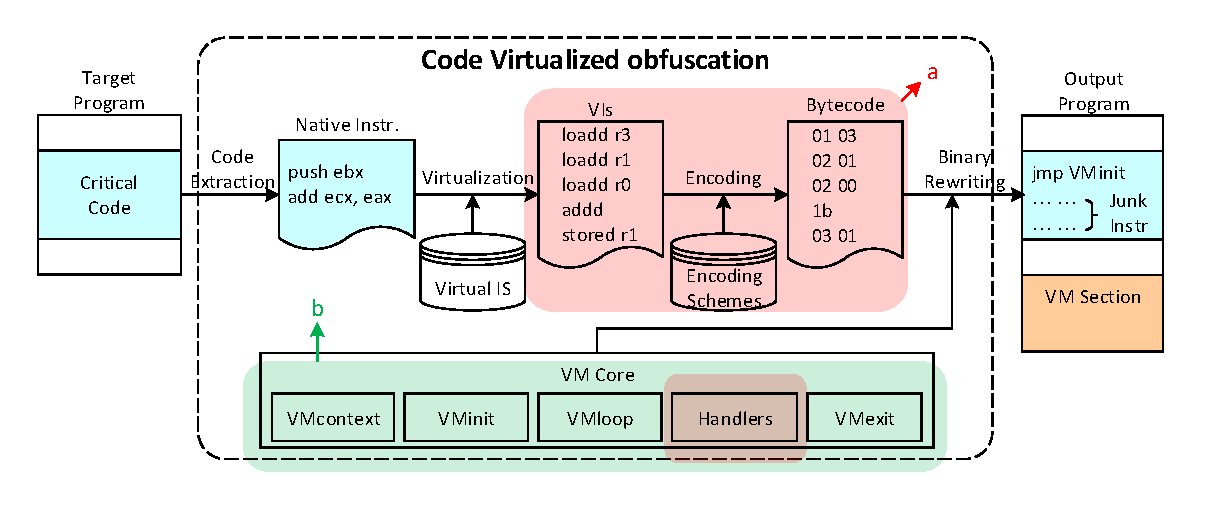
\includegraphics[width=0.9\textwidth]{fig/vmprotection.pdf}
\caption{A representative architecture for VM-based obfuscation and the execution view of a protected program. The main work of this paper is to improve the core steps of VM-based protection (areas marked as ``a" and ``b").
In the first region (a), we partition the protected code region into different segments, and obfuscate the \texttt{bytecode handlers} to generate multiple implementations for each \texttt{handler}.
In the second region, we use a number of obfuscation and anti-taint analysis technologies to protect the important components of the virtual core.}
\FIXME{Delete steps 1-4 and the left-most box. These terms are not referred anywhere in the paper.}
\label{fig:vmprotection}
\end{figure}

%Virtualization technique has been used in many fields, e.g.
%virtual memory for resource virtualization, VMware and VirtualBox for CPU virtualization,
%and Java bytecode and .Net CIL for application virtualization.
Visualization techniques is widely used to protect software programs from unauthorized analyses.
Examples of VM-based code obfuscation tools include VMProtect~\cite{vmp}, Code Virtualizer~\cite{cv} and~\cite{Themida}.
Code obfuscation often comes at a cost, with bloating code size and longer execution time.
To minimize the overhead, in practice only critical parts of the software will be obfuscated~\cite{geneiatakis2012adaptive}.
VM-based  protection works by transforming the native machine code of the protected code region into
a set of bespoke virtual instructions (bytecode), which hopefully is unknown to the attacker.
At runtime, the virtual instructions will be translated into native code using byte interpreters.



Figure \ref{fig:vmprotection} illustrates a classical VM-based obfuscation system.
At the heart of this system are the virtual IS (Instruction Set) and the set of interpreters used
to translate the IS to native code.
Interpretation of virtual instructions follows the classical \textit{decode-dispatch} approach \cite{ghosh2012replacement},
using a bundle of \texttt{handlers} and a \texttt{VMloop}.
Here, the \texttt{VMloop} is the execution engine which fetches and decodes a bytecode instruction and then dispatches a \texttt{handler} to interpret instruction.
Bytecode instructions are compiled for a virtual context,  \texttt{VMcontext}, which contains hardware-independent virtual registers and flags.
At runtime, the virtual registers and flags will be mapped down to the underlying hardware.
This work targets two key components of the VM-based obfuscation architecture, highlighted as two regions Figure \ref{fig:vmprotection} (a and b).
Our approach divides the protected code region to different sections. It generates
multiple implementations for each bytecode handler using code obfuscation techniques. Different implementations
of the same bytecode handler will produce an identical output for a given virtual instruction, by they follow different execution paths and exhibit
diverse behavior during runtime. We further enhance the strength of the protection by using a number of obfuscation and anti-taint analysis technologies to protect the important components of the VMCore.



%Figure \ref{fig:vmprotection} also depicts the workflow of the obfuscation
%process. The process starts from extracting the critical code from the target
%program. This is typically done with the help of the developer who will
%mark the location and scope of the critical code to be protected during
%the development stage. The critical code section is disassembled into
%native disassembly instructions to enable later conversion from native
%instructions to virtual instructions. The rules of conversions are set ahead of time and are often fixed
%inside a VM-based obfuscation system. These rules depend on the semantics of
%the virtual IS. Subsequently, virtual
%instructions are encoded into bytecode program. Finally, the bytecode program
%and other VM components are assembled into the target program through binary
%rewriting. This paper improves the core steps of code virtualization
%protection. We modify the encoding schemes and adopt the partition bytecode
%programming, and generate multiple sets of \texttt{handlers}. So the
%bytecodes will have different semantics in different parts of bytecode
%program. We also use a variety of methods of obfuscation and anti-taint
%analysis technology to protect the critical components of virtual interpreter
%(section~\ref{sec:VI-Bytecode}).
%
%At runtime, upon executing the ``critical code", an instruction, \texttt{jmp VMinit}, transfers the control to \texttt{VMinit} (Step \ding{182}). \texttt{VMinit} saves the native context and initializes the virtual context. Next, \texttt{VMloop} starts to work. It fetches a bytecode instruction, decodes it (Step \ding{183}) and dispatches a \texttt{handler} to interpret it (Step \ding{184}). Step \ding{183} and Step \ding{184} are iterated until all the bytecode instructions are interpreted. Then, \texttt{VMloop} transfers the execution to \texttt{VMexit} (Step \ding{185}), where the native context is restored and the program jumps back to the native instruction following the critical code (Step \ding{186}) and continue to execute the rest of the program code.

%\FIXME{I think we really need to avoid jargons here!! Everything can be explained by two short paragraphs.}
